\documentclass[12pt]{article}
\usepackage[utf8]{inputenc}
\usepackage{amsmath,amssymb}
\usepackage[T2A]{fontenc}
\usepackage[russian]{babel}
\usepackage{graphicx}
\usepackage{subfigure}
\usepackage{url}

\DeclareGraphicsExtensions{.pdf,.png,.jpg}
\usepackage{hyperref}
\usepackage{wrapfig}
\usepackage[left=20mm, top=20mm, right=10mm, bottom=20mm]{geometry}

\usepackage{amsmath} 
\usepackage{amsfonts} 
\usepackage{amssymb} 
\usepackage{wasysym} 
\usepackage{fancyhdr}

\usepackage[labelsep=period]{caption}

\pagestyle{fancy}
\fancyhf{}
\lhead{Семинар 3. Соотношение неопределенностей}
\rhead{\textit{Клименок К.Л., МФТИ 2020}}
\rfoot{\thepage}


\begin{document} 

\title{\textbf{Семинар 3. Корпускулярно-волновой дуализм. Соотношение неопределенностей}}
\author{\textbf{Клименок Кирилл Леонидович}}
\date{12.06.2020}
\maketitle

\section{Теоретическая часть}

\subsection{Корпускулярно-волновой дуализм}
На прошлой неделе мы с вами говорили о том, что световая волна может проявлять свойства частицы-фотона и взаимодействовать с другими частицами, например рассеиваться на свободных электронах (эффект Комптона). А может ли это работать и в обратную сторону, когда частица также будет проявлять волновые свойства? Если ответить на этот вопрос положительно, то окажется, что можно будет наблюдать такие явления как интерференция и дифракция для <<обычных>> частиц. Но перед этим я предлагаю оценить масштабы длин волн, с которыми нам придется иметь дело. 

\vspace{1em} \noindent
Из прошлых недель мы знаем, что энергия и импульс фотонов связаны следующими соотношениями:
\begin{equation*}
    p = \dfrac{E}{c}; \;\; E = \hbar \omega
\end{equation*}
Из этих двух соотношений мы вполне спокойно можем вытащить импульс и попреобразовывать его:
\begin{equation}
    p = \dfrac{\hbar \omega}{c} = \hbar k = \dfrac{h}{\lambda}
\end{equation}
Здесь $k$ --- волновой вектор, $\lambda$ --- длина волны. Вот мы и получили необходимую нам связь. Теперь мы можем оценить характерные длины волн. Возьмем классический пример электрона, разогнанного в поле с напряжением $U=100$ В, и подставим в полученное выражение:
\begin{equation*}
    \lambda = \dfrac{h}{m_eV} = \dfrac{h}{\sqrt{2m_eeU}} \approx \dfrac{10^{-34}}{\sqrt{10^{-31}\cdot10^{-19}\cdot10^{2}}} \text{ м} \approx 10^{-10} \text{ м}
\end{equation*}
Характерное число в 1 \AA, получается, примерно совпадает с длиной волны рентгена, а он, как, я надеюсь, вы помните из оптики, отлично дифрагирует на кристаллических решетках твердых тел. Напомню основное соотношение при такой дифракции. Пусть пучок электронов (или рентгеновское излучение) падает на плоскость кристалла под углом скольжения $\theta$, и расстояние между такими плоскостями --- d. Тогда направление на максимумы интенсивности определяется соотношением Брэгга-Вульфа: 
\begin{equation*}
    2d\sin{\theta} = n\lambda
\end{equation*}
Такой опыт по дифракции электронов был проведен Дэвиссоном и Джермером, за что в 1937 году Дэвиссону была присуждена Нобелевская премия.

\vspace{1em} \noindent
В качестве еще одного доказательства волновой природы электрона можно привести эксперименты Hitachi (1989) или Баха (2013),  которые, по своей сути, повторяли классический опыт Юнга с интерференцией на 2 щелях. Очень слабый ток электронов проходил через специальную фокусирующую систему, и в эксперименте отслеживалась точка попадания электрона на экран. Так как ток был очень слабый, можно было считать, что электроны проходили через систему по-одному. На самом экране в начале эксперимента казалось, что точки попадания случайны, но при накоплении статистики оказывалось, что здесь присутствуют полосы с большей переменной концентрацией электронов --- то есть, опыт Юнга повторялся. 

\vspace{1em} \noindent
И вот тут становится по-настоящему интересно, что происходит, и на чем же интерферирует электрон. Здесь и заканчивается классическое представление об электроне как о частице с нарисованным минусом, и подключается чисто квантовое описание электрона как волнового пакета, который, проходя через 2 щели, находится в обеих и интерферирует сам с собой. Здесь я не претендую на хорошее и строгое описание, а пытаюсь максимально просто донести саму идею. Ссылка на оригинальную статью Баха с видео формирования интерференционной картины электронов: \url{http://stacks.iop.org/NJP/15/033018/mmedia}.
\begin{figure}[h]
    \centering
    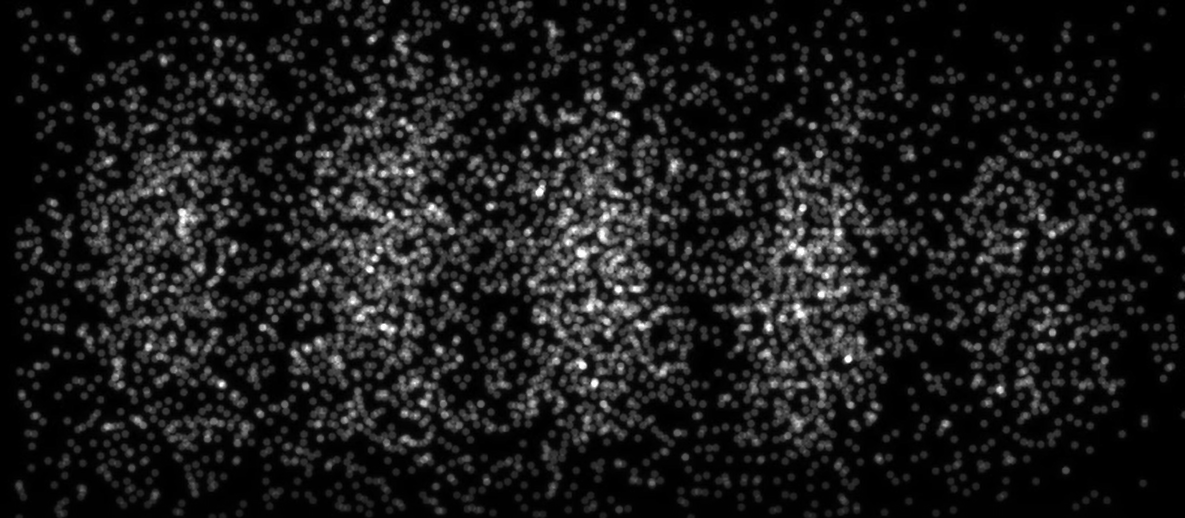
\includegraphics[width=\textwidth,height=\textheight,keepaspectratio]{Seminar_03/pics/pic_01.png}
    \caption{Распределение попадания электронов в эксперименте Баха. Каждая точка соответствует задетектированному электрону.}
    \label{fig:sem_03_bach_experiment}
\end{figure}

\subsection{Проблема измерения. Соотношение неопределенностей}
С этими новыми <<волновыми>> электронами мы получили довольно занимательное противоречие нашему предыдущему опыту: как это так, электрон --- и частица, и волна, и при этом проявляет только какое-то одно из свойств в зависимости от экспериментов. На деле, объяснить это достаточно просто, но нужно пойти к самым истокам нашего изучения физики, а именно к измерению. Рассмотрим простой пример измерения положения объекта в пространстве. Для этого нанесем в нашем пространстве сетку координат (или просто положим линейку) и осветим наш объект, чтобы мы могли увидеть, куда падает тень, и где сам объект относительно линейки. В классической физике и вашем 2-х летнем опыте физического практикума это кажется настолько естественным, что и в случае с отдельным электроном этот трюк вполне можно провернуть. На деле же, как только мы освещаем наш электрон, фотоны сталкивающиеся с ним, немного меняют его импульс, и он начинает куда-то двигаться. Аналогичная проблема возникает, если мы пытаемся измерить импульс --- становится непонятно, где же конкретно этот электрон.
\begin{figure}[h]
    \centering
    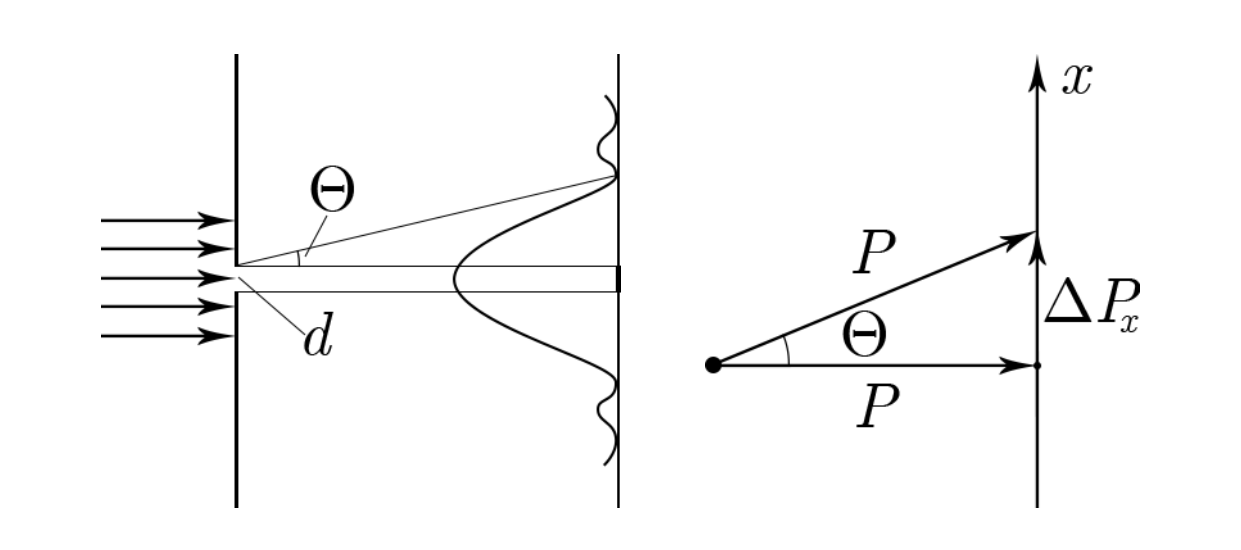
\includegraphics[width=0.7\textwidth,keepaspectratio]{Seminar_03/pics/pic_02.png}
    \caption{Схема эксперимента по дифракции электронов на щели и для вывода соотношения неопределенностей}
    \label{fig:sem_03_electron_diffraction}
\end{figure}

\noindent
Давайте рассмотрим простой пример с дифракцией электрона на отдельной щели определенной ширины. Пусть он летит на щель шириной $d$ с импульсом $p$ перпендикулярно ей. Это означает, что его длина волны $\lambda = h/p$, а из курса оптики, я надеюсь, вы помните, что направление на дифракционный минимум зависит от длины волны и ширины щели: $\sin{\theta} = \lambda/d$. То есть, у нашего электрона из-за щели появилась <<неопределенная>> составляющая импульса $\Delta p$, которая его и отклонила от своей начальной траектории. Из геометрии понятно, что $\sin{\theta} = \Delta p / p$, и отсюда окончательно можно сказать, что $d\Delta p = h$. А если мы будем рассматривать нашу щель как попытку локализовать электрон в определенном месте пространства, то ширина щели и будет, по сути, <<неопределенностью>> по координате. Окончательно мы можем записать соотношение неопределенностей следующим образом:
\begin{equation}
    \Delta p_x \Delta x \sim h
\end{equation}
Это соотношение прекрасно подходит для характерных оценок в задачах текущего семинара. Более точная запись соотношения неопределенностей представляет из себя связь дисперсий импульса и координаты, и записывается в форме Вейля:
\begin{equation*}
    \sigma^2_p \sigma^2_x \ge \dfrac{\hbar^2}{4}
\end{equation*}
И еще пара ремарок относительно полученных выражений. Во-первых, соотношение неопределенностей напрямую следует из волнового описания частиц и Фурье-анализа (пока я специально не акцентировал на этом внимания и не записывал $\psi$-функцию в явном виде, сейчас нам это не нужно). Но чтобы освежить в памяти смысл неопределённостей частота-время, я, как всегда, оставлю ссылку на видео 3Blue1Brown: \url{https://www.youtube.com/watch?v=MBnnXbOM5S4}. Во-вторых, довольно легко математическими преобразованиями получить не только соотношение импульс-координата, но и энергия-время: $\Delta E \Delta t \sim h$, если $\Delta p$ и $\Delta x$ --- неопределенности в один и тот же момент времени, а в формуле для неопределенности по энергии сама энергия измеряется в разные моменты времени. То есть, в действительности присутствует огромная разница между физическими смыслами в двух разных соотношениях неопределенностей --- для энергии и времени, и для
координаты и импульса. Одно из самых ярких примеров использования этого соотношения --- это нарушение закона сохранения энергии на масштабе времен $\Delta t$. Это нам понадобится, когда мы будем говорить о виртуальных частицах.


\section{Практическая часть}

\subsection{Задача 2.15}
\label{task_2.15}
\paragraph{Условие}
Чтобы получить пучок нейтронов, обладающих заданной энергией $E = 1$ эВ, используют брэгговское отражение первого порядка от кристалла LiF, для которого расстояние между плоскостями решетки $d = 2.32$ \AA . На кристалл падает пучок нейтронов с различными энергиями. Оценить разброс нейтронов по энергиям в отраженном пучке, если его угловая ширина $\Delta \varphi = 0.1^{\circ}$. Какую толщину кристалла D следует выбирать в этом эксперименте?
\paragraph{Решение}
На самом деле, эта задача больше на оптику, чем на кванты, так что давайте вспоминать все, что мы оттуда помним. Запишем условие Брэгга-Вульфа и оценим масштаб бедствия по углам отклонения:
\begin{gather*}
    \sin{\varphi} = \dfrac{\lambda}{2d}\\
    \lambda = \dfrac{h}{p} = \dfrac{h}{\sqrt{2mE}} \approx 0.287 \text{ \AA} \\
    \sin{\varphi} \approx \varphi \approx 0.06
\end{gather*}
Как и должно было случится, мы получили малые углы. Теперь давайте сориентируемся, как будет влиять изменение угла на изменение энергии. Выше мы увидели следующую закономерность: $\lambda \sim \varphi  \sim E^{-1/2} $. Отсюда и будет следовать:
\begin{equation*}
    \dfrac{\Delta \lambda}{\lambda} = \dfrac{\Delta \varphi}{\varphi} = \dfrac{\Delta E}{2E}
\end{equation*}
Выражаем из этого равенства $\Delta E = 2E \dfrac{\Delta \varphi}{\varphi} \approx 0.58$ эВ.

\vspace{1em} \noindent
Остался не разобранным вопрос с толщиной. Она влияет на количество слоев и, соответственно, на количество отражений. То есть, перед нами простая дифракционная решетка с известной нам разрешающей способностью:
\begin{gather*}
    \dfrac{\Delta \lambda}{\lambda} \le R = mN = 1\cdot \dfrac{D}{d}
\end{gather*}
Окончательно, $D = \dfrac{\lambda}{2\Delta \varphi} = 82 \text{ \AA}.$

\subsection{Задача 2.43}
\label{task_2.43}
\paragraph{Условие} Оценить на основании соотношения неопределенностей радиус атома водорода в основном состоянии и энергию связи электрона в том же состоянии. Определить на основании таких же оценок размер двухатомной молекулы и энергию её основного состояния, рассматривая молекулу как одномерный гармонический осциллятор с собственной частотой $\omega_0$ и приведенной массой $\mu$.
\paragraph{Решение}
\textit{Часть 1. Атом водорода.}

\vspace{3mm} \noindent
Для начала надо определиться с тем, что подставлять в соотношение неопределенностей. Тут, так как мы просто оцениваем, в качестве неопределенности координаты мы можем взять сам радиус атома, а качестве неопределенности импульса сам импульс: $\Delta x \sim r; \; \Delta p \sim p \Rightarrow p\cdot r = \hbar $. Теперь запишем полную энергию электрона в атоме водорода:
\begin{gather*}
    E = \dfrac{p^2}{2m} - \dfrac{e^2}{r} = \dfrac{\hbar^2}{2mr^2} - \dfrac{e^2}{r}
\end{gather*}
Атом находится в основном состоянии, значит, в состоянии с минимальной энергией. Найдем минимум через производную энергии по времени:
\begin{gather*}
    \dfrac{dE}{dt} = -\dfrac{\hbar^22r}{2mr^4} + \dfrac{e^2}{r^2} = 0 \Rightarrow r = \dfrac{\hbar^2}{me^2}=0.53 \text{ \AA}
\end{gather*}
Тогда энергия основного состояния:
\begin{gather*}
     E = \dfrac{\hbar^2}{2mr^2} - \dfrac{e^2}{r} = -\dfrac{me^4}{2\hbar^2} = -13.6\text{ эВ}
\end{gather*}
Что интересно, эта оценка дает точно совпадающий с теорией Бора результат.

\vspace{6mm} \noindent
\textit{Часть 2. Квантовый гармонический осциллятор.}\vspace{3mm}\\
За этим страшным названием скрывается лишь обыкновенная двухатомная молекула. Для начала, почему и здесь тоже надо применять соотношение неопределенностей, и почему эта штука не может обладать нулевой энергией? Все просто: если бы атомы в этой молекуле не колебались, то мы бы точно знали и координату каждого из них, и импульс (который, неожиданно, 0). Теперь собственно формулки. Полная энергия для такой молекулы, с учетом соотношения в форме Вейля:
\begin{gather*}
     E = \dfrac{p^2}{2\mu} + \dfrac{kx^2}{2} = \dfrac{\hbar^2}{8\mu x^2} + \dfrac{\mu \omega_0^2 x^2}{2}
\end{gather*}
Аналогично первой части найдем минимум энергии, но для простоты будем считать производную не просто по координате, а по квадрату координаты, так как минимумы будут совпадать:
\begin{gather*}
    \dfrac{dE}{dx^2} = -\dfrac{\hbar^4}{8\mu x^4} + \dfrac{\mu \omega_0^2}{2} = 0 \Rightarrow x^2 = \dfrac{\hbar}{2\mu\omega_0} \Rightarrow E = \dfrac{\hbar\omega_0}{2}
\end{gather*}
Этот результат, оказывается, также точно совпадает со строгим решением задачи о нулевом уровне энергии квантового гармонического осциллятора.

\subsection{Задача 2.31}
\label{task_2.31}
\paragraph{Условие}
Предполагая, что ядерные силы между нуклонами обусловлены обменом квантами ядерного поля --- виртуальными пионами, оценить радиус $\Delta r$ действия ядерных сил, если известно, что энергия покоя пионов $m_{\pi}c^2 \approx 140$ МэВ.
\paragraph{Решение}
Вот тут нам и пригодится соотношение неопределенностей энергия-время. Что это за пионы, и о чем идет речь в задаче? Когда мы говорим о взаимодействии, мы рассматриваем этот процесс как обмен какими-то частицами. Как работает электромагнитное взаимодействие? Есть тело, которое заряжено. Оно испускает квант электромагнитного излучения --- фотон, он летит к другому заряженному телу, которое его поглощает и тем самым узнает о первом теле. При этом второе тело также посылает фотон, который поглощает первое тело. Это работает не только с электромагнитным, но и с другими взаимодействиями, в частности с сильным взаимодействием в атоме. А частицы такого взаимодействия называются пионами или $\pi$-мезонами.

\vspace{1em} \noindent
Теперь, когда мы разобрались с тем, что происходит, давайте запишем соотношение неопределенностей. Неопределенность по энергии --- это и есть масса нашего пиона, неопределнность по времени --- время его жизни. А максимальная скорость, с которой частица может перемещаться в нашим мире это скорость света. Отсюда и получим оценку на характерный радиус сильного взаимодействия:
\begin{gather*}
    R \le c\Delta t = c\dfrac{h}{\Delta E} = c\dfrac{h}{m_{\pi}c^2}\approx 2\cdot 10^{-13} \text{ см}
\end{gather*}

\subsection{Комментарии к задачам из задания}
\paragraph{Нулевки} В первой просто подставить в формулы, вторая, по сути, решена в \ref{task_2.43}.
\paragraph{Задача 2.10} Решена в задачнике.
\paragraph{Задача 2.15} Решена, см. \ref{task_2.15}.
\paragraph{Задача 2.26} Задачка ультра-релятивистская, так что надо использовать формулу для полной энергии именно как корень, а дальше все получится.
\paragraph{Задача 2.30} Часть решения я демонстрировал в теоретической части, а часть это просто оптика.
\paragraph{Задача 2.38} Задача подозрительно напоминает часть 1 из \ref{task_2.43}.
\paragraph{Задача 2.44} Решена в задачнике.

\end{document}
